\documentclass[11pt,a4paper]{article}

\usepackage[margin=1in]{geometry}
\usepackage{graphicx}
\usepackage{hyperref}
\usepackage{amsmath,amssymb}
\usepackage{mathtools}

\title{Construction project dependency networks compress exponentially into
logical-depth levels whose mean distance to project completion is nearly
independent of project size}

\author{Alexei Vazquez\\
\small Nodes \& Links Ltd, Salisbury House, Station Road, Cambridge, CB1 2LA, UK\\
\small \texttt{alexei@nodeslinks.com}}

\date{}

\begin{document}

\maketitle

\begin{abstract}
Dependency networks link activities, events or processes by prerequisite relationships. Real dependency networks are often too large to interpret directly. We ask how to summarise them at a higher level of organisation, using construction project schedules as a case study. We introduce two deterministic groupings of activities. The Dependency Uprise Structure (DUS) collects activities with the same logical depth in the network. The Dependency Predecessor Structure (DPS) refines the DUS by also recording which earlier levels each activity depends on. We analyse 1198 construction project schedules from three companies, with 36 to 150{,}692 dependencies. The number of DUS levels grows logarithmically with the number of dependencies. The number of DPS classes grows as a sub-linear power law with exponent $0.71$ (95\% CI $[0.69, 0.72]$). Model selection favours these two forms over the alternatives we tested, and the logarithmic coefficient and the power-law exponent do not differ significantly between companies. The DUS therefore compresses the dependency network exponentially, and the DPS gives an intermediate, sub-linear summary. The mean distance from a DUS level to the end of the project is almost independent of project size, because dependencies that skip levels act as shortcuts. A degree-preserving null model shows that this follows from the degree distributions of the DUS network, not from a special arrangement of the shortcuts. The qualitative results hold on the public PSPLIB benchmark. Dependency networks also arise in causal inference, ancestry analysis and neural networks, where the same approach applies. A Python implementation is available at \url{https://github.com/av2atgh/dus} (archived at \href{https://doi.org/10.5281/zenodo.XXXXXXX}{doi:10.5281/zenodo.XXXXXXX}).
\end{abstract}

\section*{Introduction}

Most large human endeavours are organised as projects \cite{jensen16, schoper2017projectification, wagner2021projectification}. Buildings, software and new drugs are all delivered by coordinating many smaller activities under shared deadlines and budgets. The products differ, but the logistics are similar, and project management has developed as a discipline to plan and control them.

Coordinating a project requires a framework that connects daily execution with strategic goals \cite{pmi2021pmbok, taxen2011system}. The usual approach is to break the total work into smaller units that can be assigned to teams, costed, scheduled and tracked. How the work is broken down determines how progress is monitored and how risks are found.

The standard tool for this decomposition is the Work Breakdown Structure (WBS) \cite{pmi2021pmbok}. The WBS is a tree of deliverables. The final product sits at the top and is divided recursively until the leaves are activities small enough to schedule and budget individually. Figure \ref{schematic}A shows a small example for a house: the project divides into substructure, superstructure and services, and these divide into the activities that appear on the schedule. Real construction WBSs have the same form but tens of thousands of leaves.

The WBS states what needs to be done, but not in which order. To build a schedule, the project manager must specify which activities are prerequisites for which others. For example, the foundations must be poured before the frame goes up. The set of prerequisite relationships forms a {\em dependency network} (Figure \ref{schematic}B). The critical path, the slack and the expected end date are computed from this network \cite{kelley1959cpm}.

Formally, a dependency network is a directed graph \cite{gross2005graph}. Each node is an activity, and a link $A \to B$ means that activity $A$ must finish before activity $B$ can start. The network must be acyclic, since a loop $A \to B \to C \to A$ would require $A$ to finish before it starts. Dependency networks are therefore directed acyclic graphs (DAGs). Every DAG has a {\em topological order}, in which each activity comes after all its predecessors and before all its successors. In a chain $A_{1} \to A_{2} \to \dots \to A_{n}$ the order is fixed. If instead $A_{1}$ feeds both $A_{2}$ and $A'_{2}$, and both must finish before $A_{3}$ starts, then $A_{2}$ and $A'_{2}$ can be swapped. Two such nodes are {\em incomparable}: neither is an ancestor of the other. DAGs also represent causal models, ancestries and feedforward neural networks, so the constructions below are not specific to construction.

Project teams thus have two views of their work: the deliverable hierarchy of the WBS and the prerequisite wiring of the dependency network. The two views rarely agree, because dependencies cross WBS branches. In Figure \ref{schematic}, Utilities belongs to the services branch but depends on Excavate, which belongs to the substructure branch. What is missing is a high-level summary derived from the dependency network itself rather than imposed from above. This is an inverse problem: we start from the fine-grained dependencies and look for their large-scale organisation.

Several fields have addressed related problems. In project management and engineering design, the Design Structure Matrix (DSM) stores dependencies as a square matrix, which is reordered and clustered to find tightly coupled blocks of work and to sequence them \cite{steward1981dsm, browning2001dsm, eppinger2012dsm}. DSM sequencing and the layering used here both look for an order compatible with the dependencies. DSM methods, however, are mostly applied to networks with cycles, where the aim is to find and break feedback loops, and DSM clustering optimises an objective with tunable parameters. The constructions below apply to acyclic networks, have no free parameters, involve no optimisation, and aim at compression rather than resequencing. In computer science, condensing a directed graph by its strongly connected components \cite{tarjan1972dfs} turns any digraph into a DAG, but leaves a DAG unchanged. Transitive reduction \cite{aho1972transitive} removes redundant edges but keeps every node. Layered graph drawing \cite{sugiyama1981, healy2013hierarchical} assigns nodes to layers by essentially the rule used below, but only as a step towards a drawing. In network science, meso-scale structure is usually inferred statistically as communities or blocks \cite{radicchi_communities_2004, newman_communities_2006, hofman_communities_2008, karrer_blockmodels_2011, peixoto2025}. Other approaches use exact symmetry \cite{macarthur2008symmetry, sanchezgarcia2020symmetry}, graph fibrations \cite{boldi2002fibration, morone2020fibrations}, latent hyperbolic geometry \cite{krioukov2010hyperbolic}, or measures of hierarchy \cite{mones2012hierarchy, corominas2013hierarchy}. These methods have rarely been applied to dependency networks. For dependency networks the problem is simpler: because the network is directed and acyclic, a high-level structure can be extracted deterministically, without statistical inference or free parameters.

Below we define the two groupings (Figure \ref{schematic}), measure how they scale on 1198 construction schedules, and measure distances in the resulting coarse-grained networks.

\begin{figure}[t]
\centering
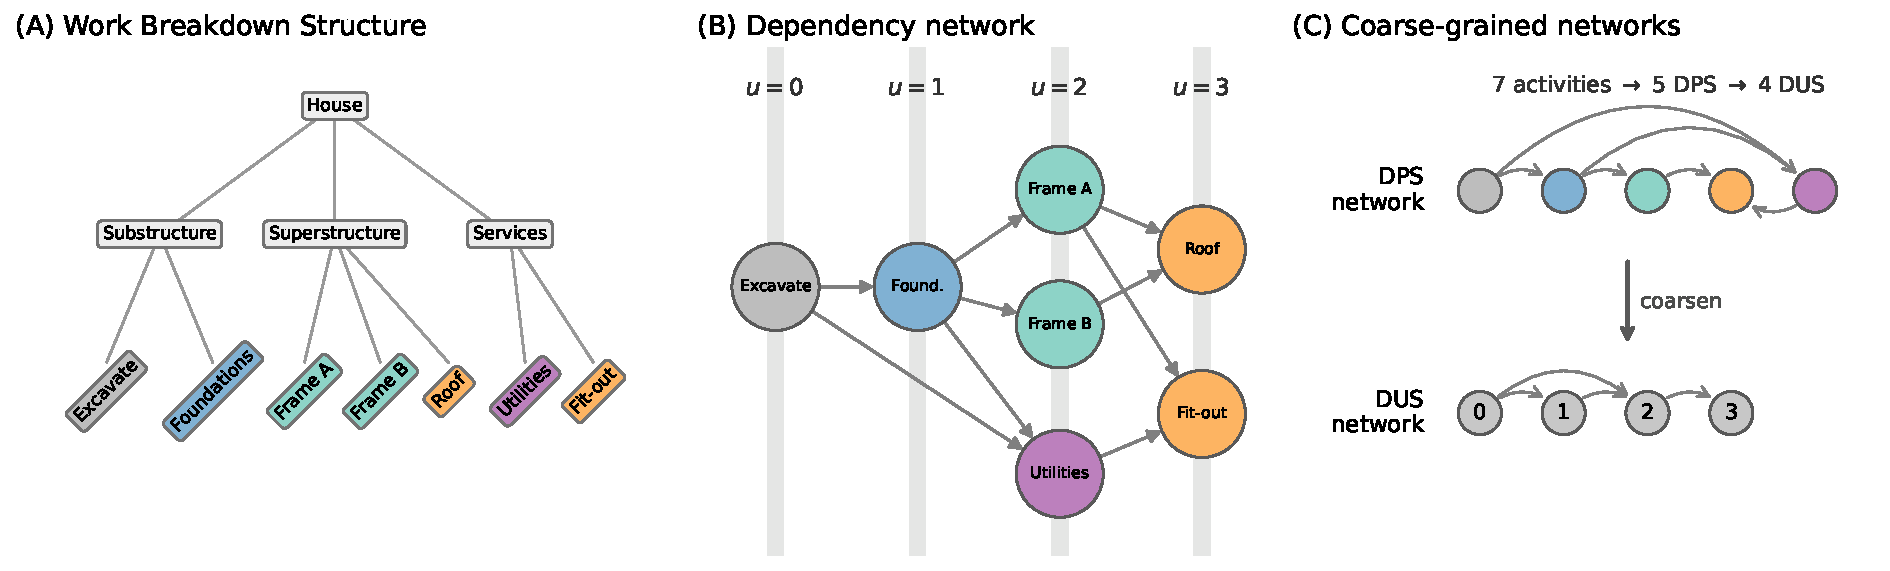
\includegraphics[width=\linewidth]{fig1.pdf}
\caption{The two coarse-grainings, illustrated on a seven-activity project. (A) A Work Breakdown Structure: the project is divided recursively into deliverables until the leaves are schedulable activities. (B) The dependency network of those activities. The DUS index $u$ of an activity is the length of the longest chain of dependencies leading to it, shown by the vertical bands. The dependency from Excavate to Utilities crosses a WBS branch. Colours indicate the DPS class, the set of DUS levels occupied by the activity's predecessors. Frame A and Frame B share a DUS level and a DPS class. Utilities is in the same DUS level but in a separate DPS class, because it also depends on level $0$. (C) The coarse-grained networks obtained by collapsing the dependency network onto DPS classes and onto DUS levels. The seven activities reduce to five DPS classes and four DUS levels.}
\label{schematic}
\end{figure}

\section*{Results}

\subsection*{Dependency Uprise Structure}

We assign each activity an integer that counts how many dependency steps separate it from a starting activity. The DUS index is $u_i = 0$ for every activity without predecessors, and otherwise
%
\begin{equation}
u_i = 1 + \max_{j\in \text{PredecessorsOf}(i)} u_j.
\label{DUS_definition}
\end{equation}
%
Evaluated in topological order, $u_i$ is the length of the longest chain of dependencies leading to activity $i$. We call it the {\em uprise} index because it measures how far the activity lies above the project start, in dependency steps rather than calendar time.

We distinguish three objects. The {\em DUS index} $u_i$ is an integer attached to each activity. A {\em DUS level} is the set of activities with the same $u_i$. The {\em Dependency Uprise Structure} (DUS) is the partition of the activities into levels. The DUS network, defined in the next section, has DUS levels as nodes.

Two activities in the same DUS level are incomparable, so they can appear in either order in a topological sort. The converse is false: activities at different depths can also be incomparable. The DUS is therefore one antichain decomposition of the DAG, and in general not the coarsest one.

Eq.~(\ref{DUS_definition}) differs from a breadth-first search from the project start, which gives the length of the {\em shortest} path from a starting activity. The two disagree when an activity has predecessors at different depths. In Figure \ref{schematic}B, a breadth-first search from Excavate places Utilities at depth $1$, because Excavate feeds it directly. Eq.~(\ref{DUS_definition}) places it at $u = 2$, because it also waits for Foundations. Only the longest-path rule places all predecessors of an activity strictly below it, so that the levels are ordered. Eq.~(\ref{DUS_definition}) also differs from a backward breadth-first search from the completion node, which would group activities by their remaining depth to the end.

Eq.~(\ref{DUS_definition}) is the layering step of the Sugiyama framework for hierarchical graph drawing \cite{sugiyama1981, healy2013hierarchical} and is related to the Coffman--Graham scheduling algorithm \cite{coffmangraham1972}. In project management terms, the DUS index of the final activity is the number of activities on the longest dependency chain, which is the critical path when all durations are equal. The layering itself is therefore not new. What is new here is its use to coarse-grain the dependency network, the empirical scaling relations below, and the finer DPS construction.

\subsection*{The DUS network}

We collapse the dependency network onto the DUS levels. In the resulting DUS network each node is a DUS level, and a weighted edge $U_a \xrightarrow{w_{ab}} U_b$ means that $w_{ab}$ activity-level dependencies run from level $a$ to level $b$. The DUS network is a DAG, like the dependency network. The weight $w_{ab}$ measures how strongly two levels are coupled.

The simplest DUS network is a chain, for example $U_0 \xrightarrow{w_{01}} U_1 \xrightarrow{w_{12}} U_2$. In general, dependencies may also skip levels. A chain through all levels is always present: by Eq.~(\ref{DUS_definition}), every activity has at least one predecessor in the previous level, so $w_{i-1,\,i} \geq 1$. The chain $U_0 \to U_1 \to \cdots \to U_{m-1}$, where $m$ is the number of DUS levels, is thus the longest path in the DUS network. We call it the {\em DUS spine}. We avoid the term critical path, which in project management refers to durations.

\begin{figure}[t]
\centering
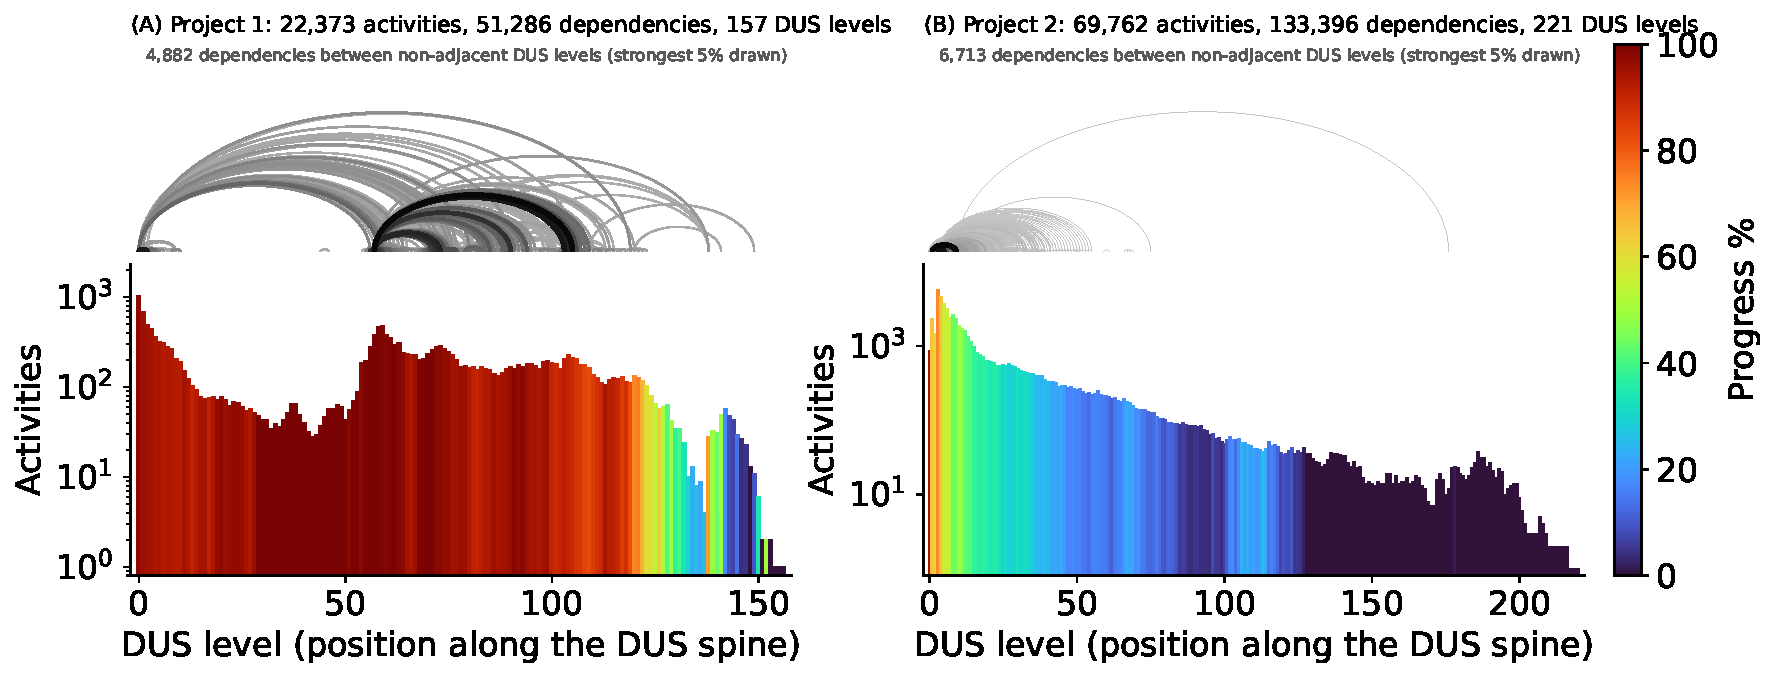
\includegraphics[width=\linewidth]{fig2.pdf}
\caption{DUS profiles of two construction project schedules. The horizontal axis is position along the DUS spine. Bars give the number of activities in each DUS level, coloured by the mean Physical Progress Percent of those activities, a standard progress metric in construction. Arcs show dependencies between non-adjacent DUS levels; darker and thicker arcs carry more dependencies. Only the strongest 5\% of arcs are drawn. Both schedules are included in the public code repository.}
\label{profiles}
\end{figure}

The DUS network has at most a few hundred nodes even for the largest schedules, so it can be drawn and used to display other project information. Figure \ref{profiles} shows the {\em DUS profile} of two construction schedules. The DUS spine runs along the horizontal axis, bar height is the number of activities in each level, colour encodes progress, and the arcs show dependencies that skip levels. A schedule of 22{,}373 activities becomes a single figure showing where the work is concentrated, how far it has progressed, and where long-range dependencies occur.

\subsection*{Scaling properties}

\begin{table}[t]
\centering
\small
\begin{tabular}{lrcccc}
\hline
 & & Activities & Dependencies & DUS levels & DPS classes \\
Company & Projects & \multicolumn{4}{c}{median [minimum--maximum]} \\
\hline
Blue & 82 & 43{,}167 [83--70{,}503] & 73{,}649 [101--137{,}450] & 170 [32--238] & 3{,}764 [35--9{,}820] \\
Green & 249 & 4{,}520 [37--104{,}981] & 7{,}284 [36--150{,}692] & 108 [17--400] & 1{,}023 [21--8{,}621] \\
Orange & 867 & 9{,}921 [37--64{,}706] & 17{,}117 [55--129{,}067] & 104 [14--571] & 1{,}079 [19--9{,}530] \\
\hline
All & 1198 & 7{,}942 [37--104{,}981] & 13{,}713 [36--150{,}692] & 108 [14--571] & 1{,}070 [19--9{,}820] \\
\hline
\end{tabular}
\caption{Descriptive statistics of the construction project schedules. The three companies are anonymised and identified by the colours used in Figures~\ref{scaling_size}--\ref{scaling_dps}.}
\label{descriptive}
\end{table}

\begin{figure}[t]
\centering
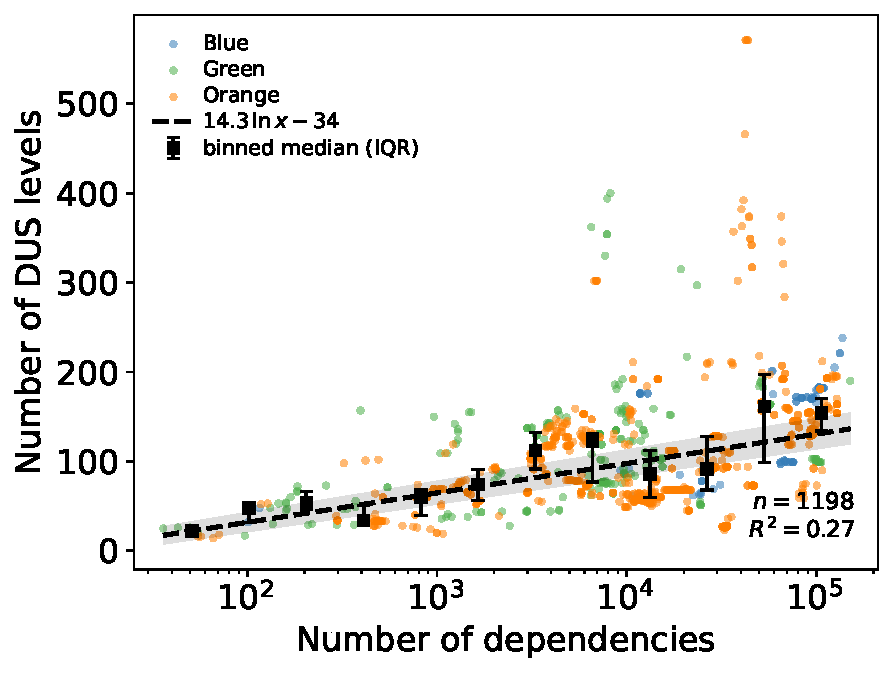
\includegraphics[width=0.62\linewidth]{fig3.pdf}
\caption{The number of DUS levels grows logarithmically with the number of dependencies. Each point is one of 1198 construction projects, coloured by company. The dashed line is the maximum-likelihood fit $m = p\ln x + c$ under multiplicative errors, with $p = 14.3$ and $c = -33.9$; the grey band is the 95\% bootstrap confidence region. Black squares are binned medians with interquartile ranges.}
\label{scaling_size}
\end{figure}

\begin{figure}[t]
\centering
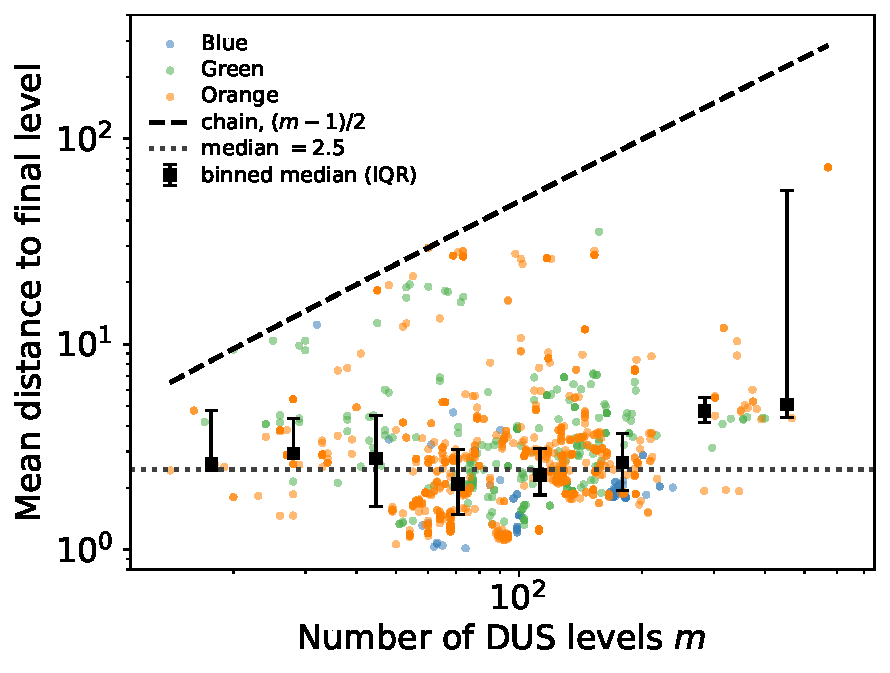
\includegraphics[width=0.62\linewidth]{fig4.pdf}
\caption{Dependencies that skip levels make the DUS network shallow. Mean shortest distance from a DUS level to the final DUS level, against the number of DUS levels $m$. The dashed line is the value $(m-1)/2$ for a pure chain. The distance is nearly independent of $m$, with median $2.5$ (dotted line). Black squares are binned medians with interquartile ranges.}
\label{scaling_distance}
\end{figure}

We collected 1198 schedules from three construction companies, labelled blue, green and orange (see Methods). Table \ref{descriptive} gives their descriptive statistics. The number of dependencies spans close to four orders of magnitude, and the size ranges of the three companies overlap substantially.

The number of DUS levels $m$ grows slowly with the number of dependencies $x$ (Figure \ref{scaling_size}). A logarithm and a power law with a small exponent are hard to distinguish over a finite range. We therefore compared four functional forms: a one-parameter logarithm, a two-parameter logarithm, a power law and a linear relation. Each was fitted by maximum likelihood with additive and with multiplicative errors and compared by AIC (Methods). The preferred model is the two-parameter logarithm with multiplicative errors, $m = 14.3\ln x - 33.9$. Its AIC is lower by $22$ than that of the power law, by $45$ than that of the one-parameter logarithm, and by $147$ than that of the linear relation. Its residuals show no detectable heteroscedasticity (Breusch--Pagan $p = 0.07$). The best power law has exponent $0.17$, which over the observed range is close to a logarithm in practice. The 95\% bootstrap confidence interval of the logarithmic coefficient is $[13.4, 15.2]$.

The relation describes the central trend, not individual projects. It explains $27\%$ of the variance in $\ln m$, and at fixed $x$ the value of $m$ varies by a factor of several. We therefore call it a logarithmic growth of the central trend rather than a scaling law. The compression is nonetheless large. A tenfold increase in $x$ adds about $33$ DUS levels at any $x$, so the DUS network is an exponential compression of the dependency network. The median project in Table \ref{descriptive} has 13{,}713 dependencies and 108 DUS levels.

Fitted separately, the three companies have logarithmic coefficients $15.9$, $16.5$ and $14.6$. We compared a model with a shared coefficient and company-specific offsets against a model with all parameters company-specific. A likelihood ratio test does not reject the shared coefficient ($\mathrm{LR} = 2.4$, $\mathrm{df} = 2$, $p = 0.30$), and AIC prefers it. The offsets differ significantly ($\mathrm{LR} = 38.4$, $\mathrm{df} = 2$, $p = 5 \times 10^{-9}$). The three companies thus share the rate $p = 15.1$, while company-specific scheduling practice shifts the number of levels.

We next measured the mean shortest distance $L$ from a DUS level to the final level. Without dependencies outside the spine, $L = (m-1)/2$. Real projects lie far below this value (Figure \ref{scaling_distance}). The median $L$ is $2.5$ levels, with interquartile range $[1.9, 3.6]$. In $99.8\%$ of projects $L$ is below $(m-1)/2$, and the median ratio is $4.6\%$. $L$ also barely grows with $m$. The binned medians are $3.4$ below $50$ levels, $2.3$ between $50$ and $150$ levels, and $2.7$ above $150$ levels, while $m$ ranges from $14$ to $571$. The rank correlation between $L$ and $m$ is small but nominally significant ($\rho = 0.10$, $p = 8 \times 10^{-4}$). With the same model selection as above, a weakly increasing linear relation is preferred over a constant ($\Delta\mathrm{AIC} = 20$), with slope $0.0041$ per level (95\% CI $[0.0018, 0.0062]$). This growth is negligible in practice. Over the observed range the fitted $L$ rises by a factor of $1.9$, from $2.5$ to $4.7$, while $m$ rises by a factor of $41$.

$L$ is small because many dependencies are shortcuts between levels far apart on the spine (arcs in Figure \ref{profiles}). Shortcuts also produce the short paths of small-world networks \cite{watts98}. For a project manager this means that a schedule with 500 DUS levels is not 500 steps deep: a few long-range dependencies connect almost any level to the end in two or three steps.

\subsection*{What makes the DUS network shallow}

\begin{figure}[t]
\centering
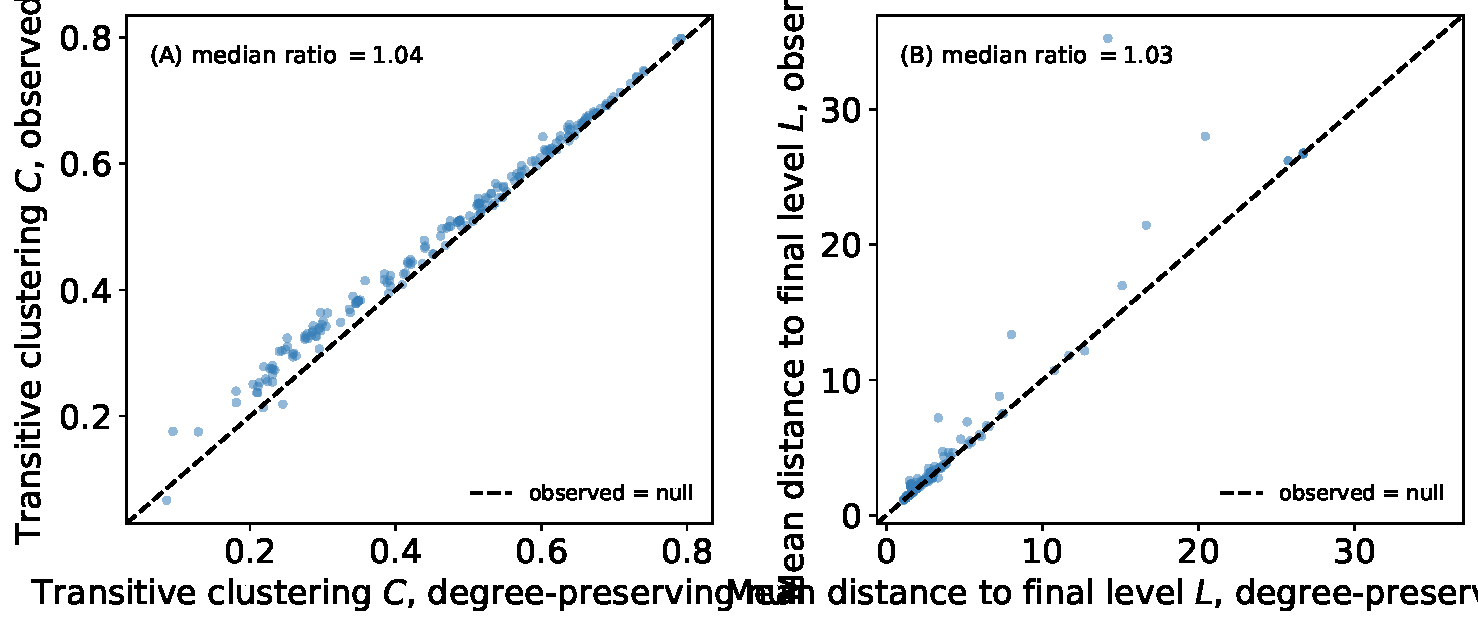
\includegraphics[width=\linewidth]{fig5.pdf}
\caption{The shallowness follows from the degree distributions. Observed versus degree-preserving null values of (A) the transitive clustering coefficient $C$ and (B) the mean distance to the final DUS level $L$, for 198 construction projects. The null keeps the DUS spine fixed and rewires the skip dependencies, preserving the skip in-degree and out-degree of every level. Each point is the average over 20 randomisations. Both quantities lie close to the identity line.}
\label{nullmodel}
\end{figure}

We tested whether the short distances require a particular arrangement of the shortcuts by comparing each DUS network with a degree-preserving null model. The usual clustering coefficient does not apply to a DAG, because a cyclic triangle is impossible. A {\em transitive} triangle, $i \to j$, $j \to k$ and the shortcut $i \to k$, is possible. We therefore use the transitive clustering coefficient $C$, the fraction of directed two-paths $i \to j \to k$ closed by an edge $i \to k$. $C$ is zero for a pure chain and increases with the number of shortcuts. The null model keeps the spine fixed, since Eq.~(\ref{DUS_definition}) forces it, and rewires the skip dependencies by double-edge swaps that preserve the skip in-degree and skip out-degree of every level (Methods).

Across 198 projects the observed values are close to those of the null model (Figure \ref{nullmodel}). The median $C/C_{\mathrm{null}}$ is $1.04$ (interquartile range $[1.01, 1.10]$) and the median $L/L_{\mathrm{null}}$ is $1.03$ (interquartile range $[1.00, 1.08]$). The short distances therefore follow from the degree distributions of the DUS network: given the number of long-range dependencies of each level, placing them at random reproduces the observed distances. The duplication-split model of activity networks \cite{vazquez2023activity} generates degree distributions of this kind, and the present result shows that these distributions are sufficient for the short distances.

The Watts--Strogatz criterion for a small world requires clustering well above that of a degree-matched null model. This excess is absent here. We therefore do not use the small-world label and state the property directly: $L$ has median $2.5$ levels, while a chain of the same depth would give up to $285$.

The degree sequence does not explain everything. A stronger randomisation preserves the in-degree and out-degree of every {\em activity}, keeps the network acyclic, and recomputes the DUS from scratch. The resulting networks are about half as deep as the real ones (median $m/m_{\mathrm{null}} \approx 2$). This ratio is a lower bound, since it grows with further randomisation. Real schedules are thus more sequential than degree-matched random DAGs. The degree distributions determine how short the paths through the DUS network are, but not how deep the network is.

\subsection*{DUS fine structure}

\begin{figure}[t]
\centering
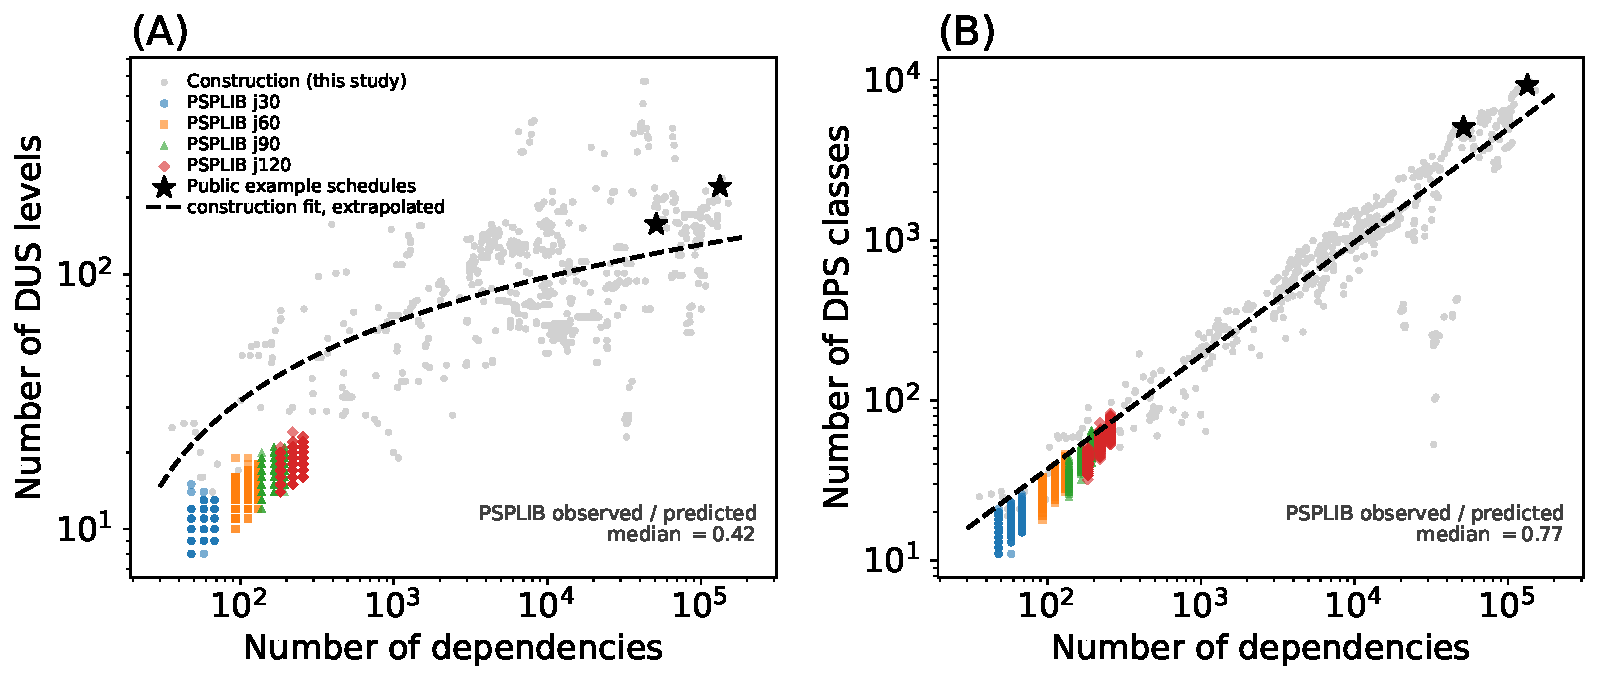
\includegraphics[width=0.62\linewidth]{fig6.pdf}
\caption{The number of DPS classes grows as a sub-linear power law with the number of dependencies. Each point is one of 1198 construction projects, coloured by company. The dashed line is the maximum-likelihood fit $1.42\,x^{0.71}$ under multiplicative errors; the grey band is the 95\% bootstrap confidence region. The dash-dotted line is a linear reference of slope $1$.}
\label{scaling_dps}
\end{figure}

Activities with the same DUS index can be split further according to the DUS levels of their predecessors (Figure \ref{schematic}B). An activity at $u = i$ has at least one predecessor at $u = i-1$, and may have predecessors at any of $u = 0, \ldots, i-2$. Each of these $i-1$ optional levels is either present or absent, so level $i$ admits $2^{i-1}$ predecessor patterns. Activities at $u = 0$ have no predecessors, and those at $u = 1$ have predecessors only at $u = 0$, so neither level can be split.

We call the resulting partition the {\em Dependency Predecessor Structure} (DPS), and each part a DPS class. As for the DUS, we distinguish the DPS index of an activity, the DPS class as a set of activities, the DPS as the partition, and the DPS network defined below. The DPS is related to {\em graph fibrations} \cite{boldi2002fibration, morone2020fibrations}. Two activities in the same DPS class have predecessors in the same set of levels. This is a local symmetry of the kind formalised by fibrations, which have been used to find building blocks of biological networks. In a DAG each class can be labelled by a single integer. We set $f_i = 0$ when $u_i = 0$ and otherwise
%
\begin{equation}
f_i= \sum_{k=0}^{u_i - 2} b_{ik}\, 2^{k} + 2^{u_i - 1}
\label{dps_definition}
\end{equation}
%
where $b_{ik}=1$ if activity $i$ has at least one predecessor in DUS level $k$ and $b_{ik}=0$ otherwise. The integer $f_i$ is a categorical label: close values of $f_i$ do not imply similar predecessor patterns.

Collapsing the dependency network onto DPS classes gives the DPS network. Each node is a DPS class, and a weighted edge $F_a \xrightarrow{w_{ab}} F_b$ counts the $w_{ab}$ activity-level dependencies between two classes. Figure \ref{scaling_dps} shows the number of DPS classes $n$ against the number of dependencies $x$. With the same model selection as above, the preferred model is a power law with multiplicative errors, $n = 1.42\,x^{0.71}$. Its AIC is lower by $269$ than that of the linear relation and by $1310$ than that of the two-parameter logarithm. The 95\% bootstrap confidence interval of the exponent is $[0.692, 0.724]$, well below $1$, and the fit explains $81\%$ of the variance in $\ln n$. The residuals are heteroscedastic, with more scatter at large $x$; for this reason the confidence interval is a case-resampling bootstrap rather than a nominal standard error. As for the DUS, a shared exponent across companies is not rejected ($\mathrm{LR} = 1.1$, $\mathrm{df} = 2$, $p = 0.59$; shared exponent $0.72$), while the prefactors differ ($p = 4 \times 10^{-6}$).

The DPS network therefore grows sub-linearly but much faster than logarithmically, and its size lies between those of the dependency network and the DUS network. The bound $2^{i-1}$ on the number of patterns at level $i$ is far from reached. A project with 100 DUS levels could have more than $10^{29}$ classes, but has of order $10^{3}$. Most combinatorially possible predecessor patterns do not occur in real schedules.

\subsection*{Replication on public data}

\begin{figure}[t]
\centering
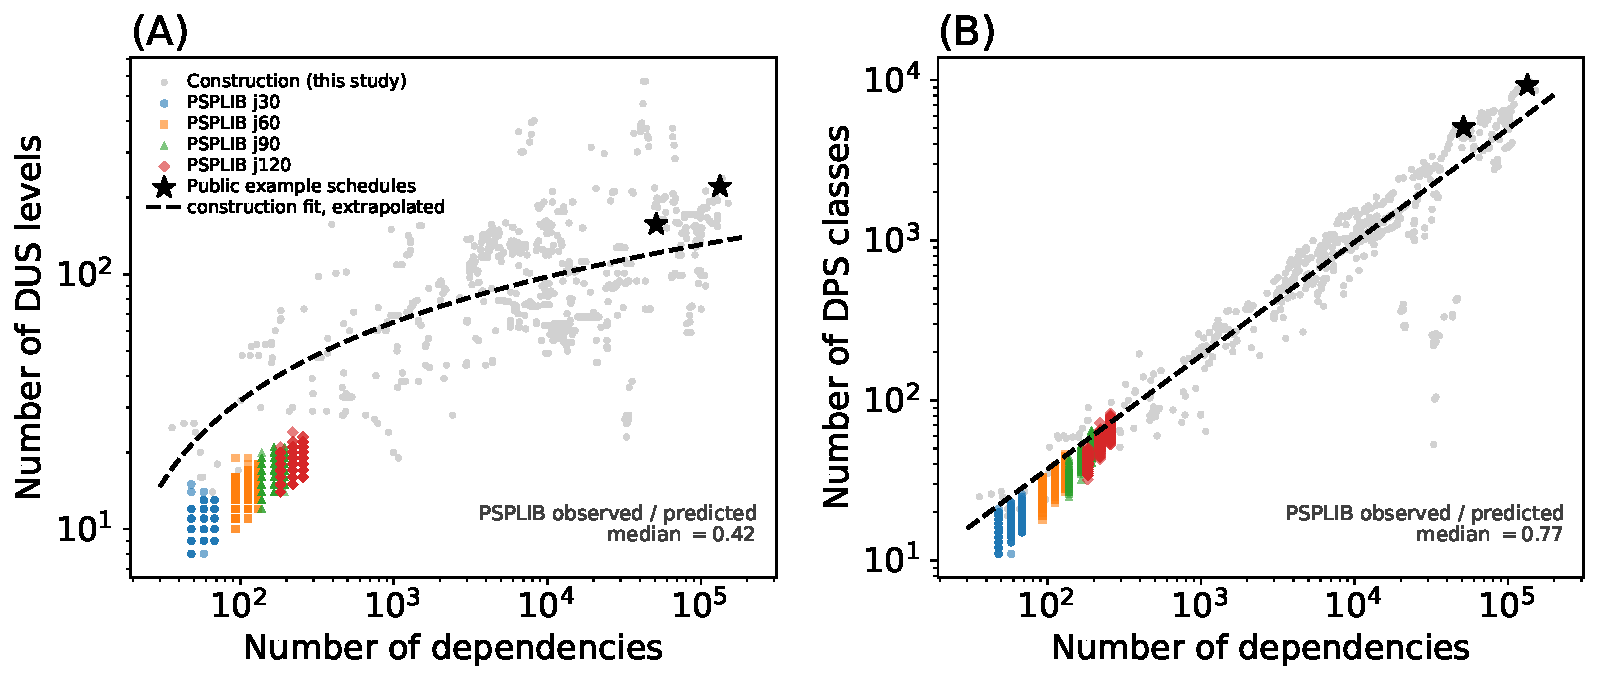
\includegraphics[width=\linewidth]{fig7.pdf}
\caption{Replication on public benchmark instances. (A) Number of DUS levels and (B) number of DPS classes against the number of dependencies, for 2040 single-mode PSPLIB instances (coloured), the 1198 construction schedules of this study (grey), and the two anonymised schedules distributed with the code repository (stars). Dashed lines are the fits to the construction data, evaluated two orders of magnitude below the median project size on which they were estimated. Only $2.4\%$ of the construction projects are as small as the largest PSPLIB instance.}
\label{public}
\end{figure}

The construction schedules are proprietary. To make the main results reproducible from public data, we repeated the analysis on the 2040 single-mode instances of PSPLIB \cite{kolisch1997psplib}, the standard benchmark library for resource-constrained project scheduling, and on the two anonymised schedules distributed with our code (Figure \ref{public}).

PSPLIB instances are much smaller than real construction schedules. They have 48 to 257 dependencies, come in only four activity counts, and span about half a decade in size. Only $2.4\%$ of our construction projects ($29$ of $1198$) are this small. Within PSPLIB alone, model selection favours a power law for the number of DUS levels and a linear relation for the number of DPS classes, unlike the construction data. With four distinct sizes over so narrow a range, we do not take this as evidence about functional form. We use PSPLIB instead to test whether the construction relations transfer to independent data at sizes where they were barely constrained.

For the DPS they do. The construction power law, evaluated two orders of magnitude below the median project size, predicts the PSPLIB values with a median observed/predicted ratio of $0.77$ (Figure \ref{public}B). A power law fitted to PSPLIB alone has exponent $0.86$, also sub-linear, although AIC does not prefer it there. For the DUS they do not. The construction logarithm over-predicts the PSPLIB values by more than a factor of two, with a median observed/predicted ratio of $0.42$ (Figure \ref{public}A). The logarithmic relation thus describes large construction schedules and is not a universal law, which is a further reason not to call it a scaling law. The qualitative result does transfer: PSPLIB DUS networks are also shallow. Their median $L$ is $2.1$, and every instance lies below the chain value.

\section*{Discussion}

Dependency networks admit two higher-level representations, which form a chain of increasingly coarse views, $\textit{Activity} \to \textit{DPS} \to \textit{DUS}$. For construction schedules, the DPS is a sub-linear coarse-graining and the DUS an exponential one.

For project management, these constructions give a view of the schedule that the WBS does not. A WBS reports progress by deliverable. The DUS reports it by logical depth, which determines what can start next. We see three uses. First, reporting: the DUS profile (Figure \ref{profiles}) reduces a schedule of tens of thousands of activities to about a hundred nodes, on which progress, cost or risk can be displayed, and a stalled level or a large concentration of work is easy to see. Second, diagnosis: the arcs in Figure \ref{profiles} are dependencies that jump many levels, and their delays propagate furthest. Each such dependency is either a real structural constraint or an artefact of how the schedule was built, and is worth checking. Third, risk modelling: a network of a hundred nodes can be simulated where one of a hundred thousand cannot. Because the compression is deterministic and has no parameters, two planners applying it to the same schedule get the same result. This is not the case for clustering methods that depend on an objective function or a random seed.

The work has three limitations. First, the relations are established on schedules from three companies in one sector, and the logarithmic relation does not extrapolate to PSPLIB, so the coefficients are not universal. Second, the DUS is one antichain decomposition among many, and we have not shown it to be optimal by any criterion. We use it because it is canonical, cheap to compute and easy to interpret. Third, each null model randomises one structure while holding either the DUS spine or the activity degree sequence fixed. The null models show what those constraints alone imply; they do not explain how real schedules acquire their degree distributions.

The construction uses only the network topology, so it applies to any system represented by a DAG, including causal networks, ancestries and feedforward neural networks. This raises three questions. Do the size relations found for construction schedules hold in those systems, and if the coefficients differ, what do the differences measure? Which features of a dependency network determine the structure of its DPS and DUS networks? The degree distributions of the DUS network account for its short distances but not its depth; which generative mechanism sets the depth? The duplication-split model \cite{vazquez2023activity} is a candidate, because its split operation creates the sequential structure that the degree-preserving null model removes.

\section*{Methods}

\subsection*{Dataset}

The construction project schedules were taken from the Nodes \& Links database. They come from three construction companies, labelled blue, green and orange, which contribute 82, 249 and 867 projects respectively, 1198 in total. Table \ref{descriptive} gives the number of activities, dependencies, DUS levels and DPS classes for each company. One further schedule was excluded because its first DUS level connects directly to every other level, so its DUS network is a star without a spine. Activity-level dependencies and Physical Progress Percent values were taken directly from the schedules as recorded in the database.

The public replication uses the four single-mode PSPLIB instance sets j30, j60, j90 and j120 \cite{kolisch1997psplib}. These comprise 2040 instances of 32, 62, 92 and 122 activities, downloaded from the PSPLIB distribution site. The precedence relations of each instance were treated as the dependencies of a construction schedule.

\subsection*{Computation of the DUS and DPS}

The activities are first sorted into a topological order with Kahn's algorithm. Eq.~(\ref{DUS_definition}) is then applied to each activity in that order. The cost is linear in the number of activities plus the number of dependencies. Given $u_i$, the DPS index $f_i$ of Eq.~(\ref{dps_definition}) requires one more pass over the dependencies: for each activity $i$ we record which lower DUS levels its predecessors occupy and combine these bits as in Eq.~(\ref{dps_definition}). The DUS and DPS networks are obtained by collapsing the dependency network onto these labels and summing edge weights. Distances in the DUS network are unweighted directed shortest-path distances, computed by one reverse sweep over the levels.

\subsection*{Null models for the DUS network}

We used two degree-preserving randomisations, both by double-edge swaps, which
preserve in- and out-degree exactly.

The first randomises the DUS network. The spine $U_0 \to U_1 \to \cdots$
is forced by Eq.~(\ref{DUS_definition}) and is held fixed. The skip
dependencies are rewired by choosing two of them, $a \to b$ and
$c \to d$, and replacing them by $a \to d$ and $c \to b$ if both new edges
are forward skips and neither already exists. This preserves the skip
in-degree and skip out-degree of each level and keeps the network acyclic. We
used 20 swap attempts per skip edge and averaged over 20 randomisations per
project. $C$ and $L$ do not change between 5 and 80 swap attempts per edge,
so the chain is well mixed.

The second randomises the activity network. A topological order of the observed
DAG is fixed, and pairs of dependencies are swapped if both new edges point
forward in that order. This preserves the in- and out-degree of every activity
and keeps the network acyclic. The DUS is then recomputed from scratch. This
randomisation mixes more slowly: the number of DUS levels still drifts at 20
swap attempts per edge, and the gap between observed and randomised networks
widens with further mixing. The ratios reported for it are therefore lower
bounds rather than converged estimates.

The transitive clustering coefficient $C$ is the number of directed two-paths
$i \to j \to k$ closed by an edge $i \to k$, divided by the number of directed
two-paths. $L$ is the mean shortest-path distance to the final DUS level.

\subsection*{Statistical methods}

For each relation we fitted four functional forms: a one-parameter logarithm $y = p\ln x$, a two-parameter logarithm $y = p\ln x + c$, a power law $y = a x^{b}$, and a linear relation $y = ax + b$. Each was fitted by maximum likelihood with two error structures: additive, $y = f(x) + \varepsilon$, and multiplicative, $y = f(x)\,e^{\varepsilon}$, with $\varepsilon \sim N(0,\sigma^2)$ in both cases. The multiplicative log-likelihoods include the Jacobian term $-\sum_i \ln y_i$. All eight fits are then likelihoods of the same observed quantity, and their AIC and BIC values can be compared across functional forms and error structures. An ordinary least squares fit on log-log axes is not comparable in this way to a fit on the natural scale.

Confidence intervals are nonparametric case-resampling bootstraps with 2000 replicates, which do not assume homoscedastic residuals. This matters for the DPS relation, whose residuals are heteroscedastic. Heteroscedasticity was tested with a Breusch--Pagan test of the squared residuals against $\ln x$.

Differences between companies were tested with nested likelihood ratio tests under the selected error structure. We compared three models: a pooled model with one shared parameter pair; a model with a shared logarithmic coefficient or power-law exponent and company-specific offsets or prefactors; and a model with all parameters company-specific. This separates whether the companies share the form of the relation from whether they share its nuisance parameters. We report the likelihood ratio statistic, its degrees of freedom, its $p$ value and the AIC of each model.

We did not apply the Clauset--Shalizi--Newman procedure \cite{clauset2009powerlaw}, which fits and tests heavy-tailed probability distributions of a single variable. The relations studied here are regressions of one measured quantity on another across projects, not distributions. The concerns about naive log-log fitting that motivate that procedure are addressed here by the error-model comparison and the bootstrap intervals.

\subsection*{Code and data availability}

The code is available at \url{https://github.com/av2atgh/dus}, and the version used for this paper is archived on Zenodo at \href{https://doi.org/10.5281/zenodo.XXXXXXX}{doi:10.5281/zenodo.XXXXXXX}. It contains a Python implementation of the DUS and DPS algorithms, the two anonymised construction schedules of Figure \ref{profiles}, code for the DUS profile plots, and the scripts that perform the statistical analysis, download and process the PSPLIB benchmark, and generate every figure in this paper. The PSPLIB instances are publicly available from \url{https://www.om-db.wi.tum.de/psplib/}. The construction project schedules are proprietary to Nodes \& Links Ltd and its clients and cannot be released. Table \ref{descriptive} gives their summary statistics, and Figure \ref{public} shows that the main results are reproducible on public data.

\section*{Acknowledgements}

This research did not receive any specific grant from funding agencies in the public, commercial, or not-for-profit sectors. Nodes \& Links Ltd provided support in the form of salary for Alexei Vazquez but did not have any additional role in the conceptualisation of the study, the analysis, the decision to publish or the preparation of the manuscript.

\section*{Author contributions}

A.V. conceived the study, designed and implemented the algorithms, performed the analysis, prepared the figures and wrote the manuscript.

\section*{Use of generative AI}

The author used Claude (Anthropic) for language editing of the manuscript text and for assistance with the statistical analysis code and figure generation scripts. The tool was not used for the conception of the study or the design of the algorithms. All analyses were verified by the author, and all scientific content, claims and conclusions are the responsibility of the author.


%\bibliographystyle{unsrt}
%\bibliography{risk}

\begin{thebibliography}{10}

\bibitem{jensen16}
Anders Jensen, Christian Thuesen, and Joana Geraldi.
\newblock The {Projectification} of {Everything}: {Projects} as a {Human}
  {Condition}.
\newblock {\em Proj. Manag. J.}, 47(3):21--34, 2016.

\bibitem{schoper2017projectification}
Yvonne-Gabriele Schoper, Andreas Wald, Helgi~Thor Ingason, and Thordur~Vikingur
  Fridgeirsson.
\newblock Projectification in western economies: A comparative study of
  germany, norway and iceland.
\newblock {\em International Journal of Project Management}, 36(1):71--82,
  2018.
\newblock Festschrift for Professor J. Rodney Turner.

\bibitem{wagner2021projectification}
Reinhard Wagner, Martina Huemann, and Mladen Radujkovic.
\newblock The influence of project management associations on projectification
  of society – an institutional perspective.
\newblock {\em Project Leadership and Society}, 2:100021, 2021.

\bibitem{pmi2021pmbok}
{Project Management Institute}.
\newblock {\em A Guide to the Project Management Body of Knowledge
  (PMBOK{\textregistered} Guide)}.
\newblock Project Management Institute, Newtown Square, PA, seventh edition,
  2021.

\bibitem{taxen2011system}
Lars Tax{\'e}n.
\newblock {\em The System Anatomy – Enabling Agile Project Management}.
\newblock Studentlitteratur, Lund, 2011.

\bibitem{kelley1959cpm}
James~E. Kelley~Jr. and Morgan~R. Walker.
\newblock Critical-path planning and scheduling.
\newblock In {\em Papers Presented at the December 1--3, 1959, Eastern Joint
  IRE-AIEE-ACM Computer Conference}, pages 160--173, New York, 1959. ACM Press.

\bibitem{steward1981dsm}
Donald~V. Steward.
\newblock The design structure system: A method for managing the design of
  complex systems.
\newblock {\em IEEE Transactions on Engineering Management},
  EM-28(3):71--74, 1981.

\bibitem{browning2001dsm}
Tyson~R. Browning.
\newblock Applying the design structure matrix to system decomposition and
  integration problems: A review and new directions.
\newblock {\em IEEE Transactions on Engineering Management}, 48(3):292--306,
  2001.

\bibitem{eppinger2012dsm}
Steven~D. Eppinger and Tyson~R. Browning.
\newblock {\em Design Structure Matrix Methods and Applications}.
\newblock MIT Press, Cambridge, MA, 2012.

\bibitem{tarjan1972dfs}
Robert Tarjan.
\newblock Depth-first search and linear graph algorithms.
\newblock {\em SIAM Journal on Computing}, 1(2):146--160, 1972.

\bibitem{aho1972transitive}
A.~V. Aho, M.~R. Garey, and J.~D. Ullman.
\newblock The transitive reduction of a directed graph.
\newblock {\em SIAM Journal on Computing}, 1(2):131--137, 1972.

\bibitem{healy2013hierarchical}
Patrick Healy and Nikola~S. Nikolov.
\newblock Hierarchical drawing algorithms.
\newblock In Roberto Tamassia, editor, {\em Handbook of Graph Drawing and
  Visualization}, pages 409--453. Chapman and Hall/CRC, Boca Raton, FL, 2013.

\bibitem{macarthur2008symmetry}
Ben~D. MacArthur, Rub{\'e}n~J. S{\'a}nchez-Garc{\'i}a, and James~W. Anderson.
\newblock Symmetry in complex networks.
\newblock {\em Discrete Applied Mathematics}, 156(18):3525--3531, 2008.

\bibitem{sanchezgarcia2020symmetry}
Rub{\'e}n~J. S{\'a}nchez-Garc{\'i}a.
\newblock Exploiting symmetry in network analysis.
\newblock {\em Communications Physics}, 3:87, 2020.

\bibitem{krioukov2010hyperbolic}
Dmitri Krioukov, Fragkiskos Papadopoulos, Maksim Kitsak, Amin Vahdat, and
  Mari{\'a}n Bogu{\~n}{\'a}.
\newblock Hyperbolic geometry of complex networks.
\newblock {\em Phys. Rev. E}, 82:036106, Sep 2010.

\bibitem{mones2012hierarchy}
Enys Mones, Lilla Vicsek, and Tam{\'a}s Vicsek.
\newblock Hierarchy measure for complex networks.
\newblock {\em PLoS ONE}, 7(3):e33799, 2012.

\bibitem{corominas2013hierarchy}
Bernat Corominas-Murtra, Joaqu{\'i}n Go{\~n}i, Ricard~V. Sol{\'e}, and Carlos
  Rodr{\'i}guez-Caso.
\newblock On the origins of hierarchy in complex networks.
\newblock {\em Proceedings of the National Academy of Sciences},
  110(33):13316--13321, 2013.

\bibitem{clauset2009powerlaw}
Aaron Clauset, Cosma~Rohilla Shalizi, and M.~E.~J. Newman.
\newblock Power-law distributions in empirical data.
\newblock {\em SIAM Review}, 51(4):661--703, 2009.

\bibitem{kolisch1997psplib}
Rainer Kolisch and Arno Sprecher.
\newblock {PSPLIB} --- a project scheduling problem library.
\newblock {\em European Journal of Operational Research}, 96(1):205--216, 1997.

\bibitem{radicchi_communities_2004}
Filippo Radicchi, Claudio Castellano, Federico Cecconi, Vittorio Loreto, and
  Domenico Parisi.
\newblock Defining and identifying communities in networks.
\newblock {\em Proceedings of the National Academy of Sciences},
  101(9):2658--2663, 2004.

\bibitem{newman_communities_2006}
M.~E.~J. Newman.
\newblock Modularity and community structure in networks.
\newblock {\em Proceedings of the National Academy of Sciences},
  103(23):8577--8582, 2006.

\bibitem{hofman_communities_2008}
Jake~M. Hofman and Chris~H. Wiggins.
\newblock Bayesian approach to network modularity.
\newblock {\em Phys. Rev. Lett.}, 100:258701, Jun 2008.

\bibitem{karrer_blockmodels_2011}
Brian Karrer and M.~E.~J. Newman.
\newblock Stochastic blockmodels and community structure in networks.
\newblock {\em Phys. Rev. E}, 83:016107, Jan 2011.

\bibitem{peixoto2025}
Tiago~P. Peixoto.
\newblock Network reconstruction via the minimum description length principle.
\newblock {\em Phys. Rev. X}, 15:011065, Mar 2025.

\bibitem{gross2005graph}
Jonathan~L Gross and Jay Yellen.
\newblock {\em Graph Theory and Its Applications}.
\newblock Chapman and Hall/CRC, Boca Raton, FL, 2nd edition, 2005.

\bibitem{sugiyama1981}
Kozo Sugiyama, Shojiro Tagawa, and Mitsuhiko Toda.
\newblock Methods for visual understanding of hierarchical system structures.
\newblock {\em IEEE Transactions on Systems, Man, and Cybernetics},
  11(2):109--125, 1981.

\bibitem{coffmangraham1972}
E.~G. Coffman and R.~L. Graham.
\newblock Optimal scheduling for two-processor systems.
\newblock {\em Acta Informatica}, 1(3):200--213, 1972.

\bibitem{watts98}
Duncan~J. Watts and Steven~H. Strogatz.
\newblock Collective dynamics of ‘small-world’ networks.
\newblock {\em Nature}, 393(6684):440--442, June 1998.

\bibitem{vazquez2023activity}
Alexei Vazquez, Iacopo Pozzana, Georgios Kalogridis, and Christos Ellinas.
\newblock Activity networks determine project performance.
\newblock {\em Scientific Reports}, 13:509, 2023.

\bibitem{boldi2002fibration}
Paolo Boldi and Sebastiano Vigna.
\newblock Fibrations of graphs.
\newblock {\em Discrete Mathematics}, 243(1):21--66, 2002.

\bibitem{morone2020fibrations}
Flaviano Morone, Ian Leifer, and Hernán~A. Makse.
\newblock Fibration symmetries uncover the building blocks of biological
  networks.
\newblock {\em Proceedings of the National Academy of Sciences},
  117(15):8306--8314, 2020.

\end{thebibliography}


\end{document}
